\documentclass[12pt]{article}

\usepackage{graphicx}
\usepackage{paralist}
\usepackage{amsfonts}
\usepackage{amsmath}
\usepackage{hhline}
\usepackage{booktabs}
\usepackage{multirow}
\usepackage{multicol}
\usepackage{url}


\oddsidemargin -10mm
\evensidemargin -10mm
\textwidth 160mm
\textheight 200mm
\renewcommand\baselinestretch{1.0}

\pagestyle {plain}
\pagenumbering{arabic}

\newcounter{stepnum}

%% Comments

\usepackage{color}

\newif\ifcomments\commentstrue

\ifcomments
\newcommand{\authornote}[3]{\textcolor{#1}{[#3 ---#2]}}
\newcommand{\todo}[1]{\textcolor{red}{[TODO: #1]}}
\else
\newcommand{\authornote}[3]{}
\newcommand{\todo}[1]{}
\fi

\newcommand{\wss}[1]{\authornote{blue}{SS}{#1}}

\title{\textbf{Machine Learning Study Notes}}
\author{Sida Wang}

\begin {document}

\maketitle
This is my personal machine learning study notes for academic purposes only.

\newpage

\section* {Linear Regression}
\begin{itemize}
\item \textbf{Supervised Learning:} Given the "right answer" for each example in the data.
\item \textbf{Two types of Supervised Learning:} Regression problem,     Classification problem.
\item \textbf{Regression Problem:} Predict real-valued output.
\item \textbf{Classification Problem:} Predict dicrete-valued output.
\end{itemize}

\subsection* {Traning Set}
 
\begin{itemize}
\item \textbf{Notation:} 
\item \textbf{m--} Number of training examples
\item \textbf{x--} "input" variable(data)
\item \textbf{y--} "output" variable(predict)
\item \textbf{(x,y)--} one training example
\item \textbf{($x^i,y^i$)--} $i^{th}$ training example
\end{itemize}

\subsection* {Supervised Learning}

    \begin{center}
    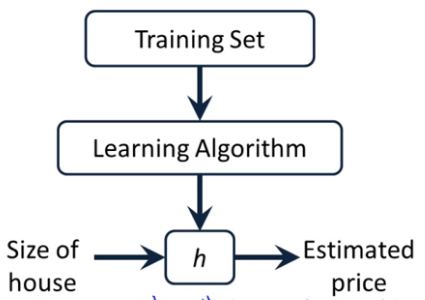
\includegraphics[scale=0.5]{SupervisedLearning.png}
    \end{center}
    The learning algorithm output a function based on the training set.\\The function h is a hypothesis that maps from x to y.

\begin{itemize}
\item \boldmath{$h_\theta(x) = \theta_0 + \theta_1x$}    (shorthand: h(x))
\item \textbf{h :} predicting y is a linear function of x, $\theta_i$s are parameters.
\end{itemize}

    \begin{center}
    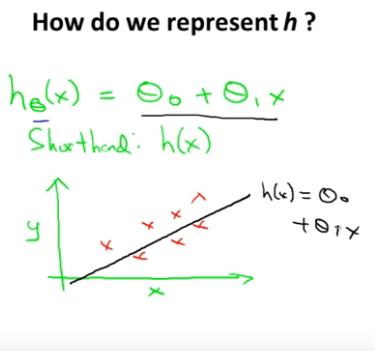
\includegraphics[scale=0.5]{UnivariateLinearRegression.png}
    \end{center}

\subsection* {Univariate Linear Regression}

    Linear regression with one variable(like above).

\subsection* {Cost Function}
    \begin{center}
    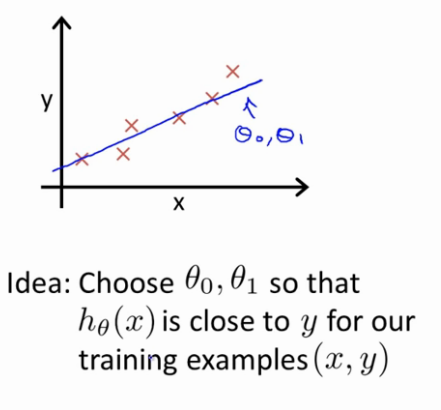
\includegraphics[scale=0.5]{ChooseTheta.png}
    \end{center}

    \begin{itemize}
    \item \textbf{Cost Function(Squared error function): } \\\boldmath{$J(\theta_0,\theta_1) = \dfrac{1}{2m} \sum_{i=1}^{m} (h_\theta(x^i) - y^i)^2$}\\\boldmath{$h_\theta(x) = \theta_0 + \theta_1x$}\\\textbf{Minimize $\theta_0$ and $\theta_1$ will minimize cost function}\\\textbf{Goal : Minimize J}\\\textbf{most commonly used for linear regression problems}

    \item \textbf{Example with $\theta_0 = 0$} 
    \begin{center}
    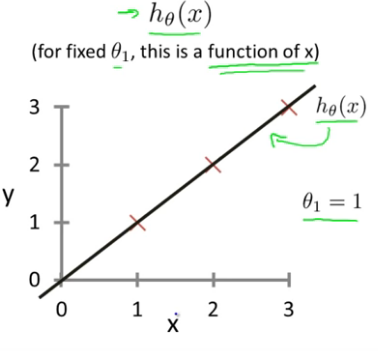
\includegraphics[scale=0.5]{Example1.png}
    \end{center}
    \boldmath{$\theta_1 = 1$}\\\\
    $J(\theta_1)  = \dfrac{1}{2m} \sum_{i=1}^{m} (\theta_1(x^i) - y^i)^2\\ 
                  = \dfrac{1}{2m} \sum_{i=1}^{m} (0^2 + 0^2 + 0^2)\\ \\
                  = 0^2$

    \begin{center}
    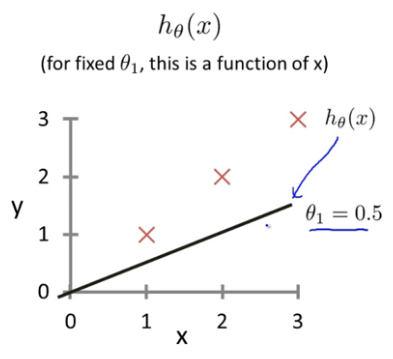
\includegraphics[scale=0.5]{Example2.png}
    \end{center}
    \boldmath{$\theta_1 = 0.5$}\\\\
    $J(\theta_1)  = \dfrac{1}{2m} \sum_{i=1}^{m} (\theta_1(x^i) - y^i)^2\\ 
                  = \dfrac{1}{2m} \sum_{i=1}^{m} ((0.5-1)^2 + (1-2)^2 + (1.5-3)^2)\\ \\
                  = \dfrac{1}{2x3} (3.5) \\ \\
                  = 0.68$
    \begin{center}
    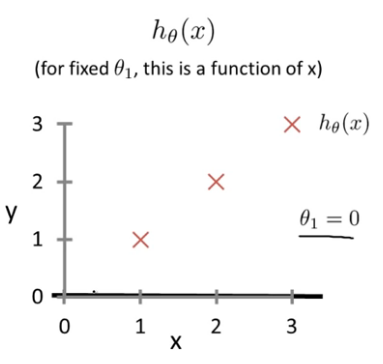
\includegraphics[scale=0.5]{Example3.png}
    \end{center}
    \boldmath{$\theta_1 = 0$}\\\\
    $J(\theta_1)  = \dfrac{1}{2m} \sum_{i=1}^{m} (\theta_1(x^i) - y^i)^2\\ 
                  = \dfrac{1}{2m} \sum_{i=1}^{m} ((0-1)^2 + (0-2)^2 + (0-3)^2)\\ \\
                  = \dfrac{1}{2x3} (14) \\ \\
                  = 2.3$\\

    \newpage
    \textbf{Using result plot cost function: } 

    \begin{center}
    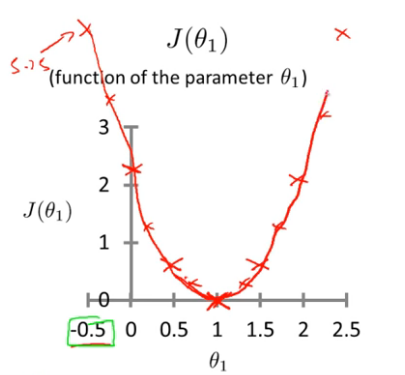
\includegraphics[scale=0.5]{Cost.png}
    \end{center}
    \textbf{The value of $\theta_1$ that minimize cost function is 1 } 
    \item \textbf{Cost function with two parameters}
    \begin{center}
    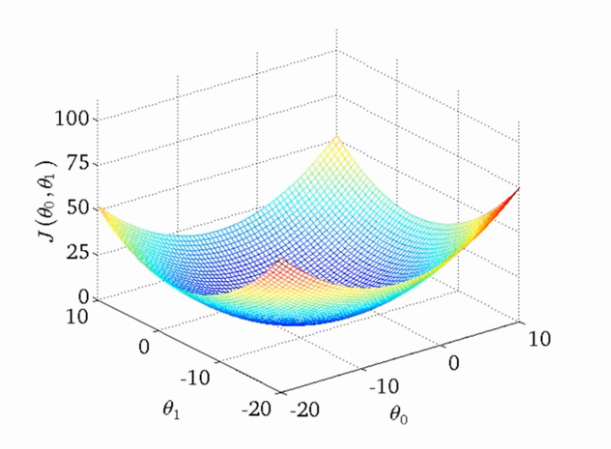
\includegraphics[scale=0.5]{Twoparameter.png}
    \end{center}
    
    \end{itemize}


\end {document}
